\documentclass{extbook}[14pt]
\usepackage{multicol, enumerate, enumitem, hyperref, color, soul, setspace, parskip, fancyhdr, amssymb, amsthm, amsmath, bbm, latexsym, units, mathtools}
\everymath{\displaystyle}
\usepackage[headsep=0.5cm,headheight=0cm, left=1 in,right= 1 in,top= 1 in,bottom= 1 in]{geometry}
\usepackage{dashrule}  % Package to use the command below to create lines between items
\newcommand{\litem}[1]{\item #1

\rule{\textwidth}{0.4pt}}
\pagestyle{fancy}
\lhead{}
\chead{Answer Key for Module6 Version A}
\rhead{}
\lfoot{9356-6875}
\cfoot{}
\rfoot{testing}
\begin{document}
\textbf{This key should allow you to understand why you choose the option you did (beyond just getting a question right or wrong). \href{https://xronos.clas.ufl.edu/mac1105spring2020/courseDescriptionAndMisc/Exams/LearningFromResults}{More instructions on how to use this key can be found here}.}

\textbf{If you have a suggestion to make the keys better, \href{https://forms.gle/CZkbZmPbC9XALEE88}{please fill out the short survey here}.}

\textit{Note: This key is auto-generated and may contain issues and/or errors. The keys are reviewed after each exam to ensure grading is done accurately. If there are issues (like duplicate options), they are noted in the offline gradebook. The keys are a work-in-progress to give students as many resources to improve as possible.}

\rule{\textwidth}{0.4pt}

\begin{enumerate}\litem{
Describe the end behavior of the polynomial below.
\[ f(x) = 8(x - 3)^{4}(x + 3)^{5}(x + 4)^{5}(x - 4)^{5} \]The solution is the graph below, which is option D.
\begin{center}
    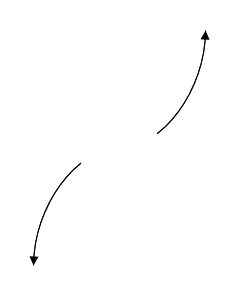
\includegraphics[width=0.3\textwidth]{../Figures/polyEndBehaviorDA.png}
\end{center}\begin{enumerate}[label=\Alph*.]
\begin{multicols}{2}
\item 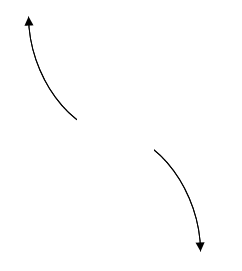
\includegraphics[width = 0.3\textwidth]{../Figures/polyEndBehaviorAA.png}
\item 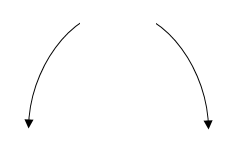
\includegraphics[width = 0.3\textwidth]{../Figures/polyEndBehaviorBA.png}
\item 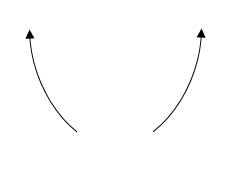
\includegraphics[width = 0.3\textwidth]{../Figures/polyEndBehaviorCA.png}
\item 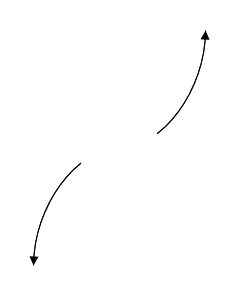
\includegraphics[width = 0.3\textwidth]{../Figures/polyEndBehaviorDA.png}
\end{multicols}\item None of the above.\end{enumerate}
\textbf{General Comment:} Remember that end behavior is determined by the leading coefficient AND whether the \textbf{sum} of the multiplicities is positive or negative.
}
\litem{
Which of the following equations \textit{could} be of the graph presented below?

\begin{center}
    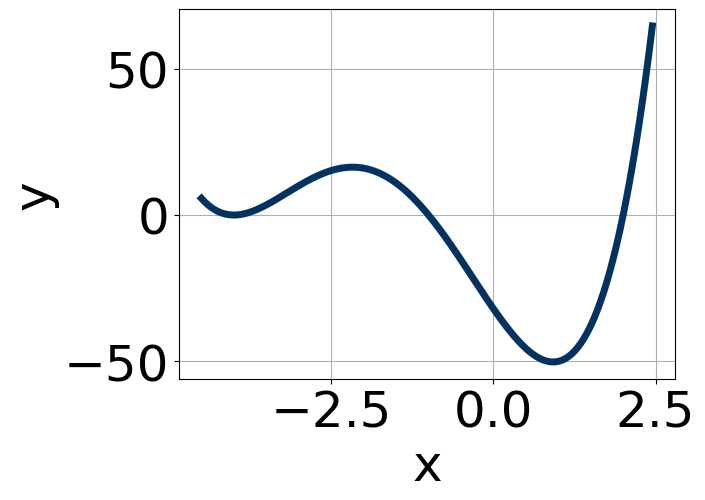
\includegraphics[width=0.5\textwidth]{../Figures/polyGraphToFunctionA.png}
\end{center}


The solution is \( 19(x + 4)^{4} (x - 2)^{7} (x + 1)^{7} \), which is option E.\begin{enumerate}[label=\Alph*.]
\item \( -4(x + 4)^{6} (x - 2)^{9} (x + 1)^{11} \)

This corresponds to the leading coefficient being the opposite value than it should be.
\item \( 16(x + 4)^{6} (x - 2)^{4} (x + 1)^{5} \)

The factor $(x - 2)$ should have an odd power.
\item \( -16(x + 4)^{10} (x - 2)^{11} (x + 1)^{10} \)

The factor $(x + 1)$ should have an odd power and the leading coefficient should be the opposite sign.
\item \( 13(x + 4)^{9} (x - 2)^{8} (x + 1)^{7} \)

The factor $-4$ should have an even power and the factor $2$ should have an odd power.
\item \( 19(x + 4)^{4} (x - 2)^{7} (x + 1)^{7} \)

* This is the correct option.
\end{enumerate}

\textbf{General Comment:} General Comments: Draw the x-axis to determine which zeros are touching (and so have even multiplicity) or cross (and have odd multiplicity).
}
\litem{
Construct the lowest-degree polynomial given the zeros below. Then, choose the intervals that contain the coefficients of the polynomial in the form $ax^3+bx^2+cx+d$.
\[ \frac{-2}{3}, \frac{3}{5}, \text{ and } \frac{2}{5} \]The solution is \( 75x^{3} -25 x^{2} -32 x + 12 \), which is option B.\begin{enumerate}[label=\Alph*.]
\item \( a \in [72, 77], b \in [-130, -118], c \in [63, 76], \text{ and } d \in [-16, -11] \)

$75x^{3} -125 x^{2} +68 x -12$, which corresponds to multiplying out $(3x -2)(5x -3)(5x -2)$.
\item \( a \in [72, 77], b \in [-30, -21], c \in [-35, -29], \text{ and } d \in [9, 15] \)

* $75x^{3} -25 x^{2} -32 x + 12$, which is the correct option.
\item \( a \in [72, 77], b \in [-38, -33], c \in [-30, -21], \text{ and } d \in [9, 15] \)

$75x^{3} -35 x^{2} -28 x + 12$, which corresponds to multiplying out $(3x -2)(5x + 3)(5x -2)$.
\item \( a \in [72, 77], b \in [24, 26], c \in [-35, -29], \text{ and } d \in [-16, -11] \)

$75x^{3} +25 x^{2} -32 x -12$, which corresponds to multiplying out $(3x -2)(5x + 3)(5x + 2)$.
\item \( a \in [72, 77], b \in [-30, -21], c \in [-35, -29], \text{ and } d \in [-16, -11] \)

$75x^{3} -25 x^{2} -32 x -12$, which corresponds to multiplying everything correctly except the constant term.
\end{enumerate}

\textbf{General Comment:} To construct the lowest-degree polynomial, you want to multiply out $(3x + 2)(5x -3)(5x -2)$
}
\litem{
Construct the lowest-degree polynomial given the zeros below. Then, choose the intervals that contain the coefficients of the polynomial in the form $x^3+bx^2+cx+d$.
\[ -4 - 5 i \text{ and } 1 \]The solution is \( x^{3} +7 x^{2} +33 x -41 \), which is option D.\begin{enumerate}[label=\Alph*.]
\item \( b \in [-11, -2], c \in [30.6, 36.6], \text{ and } d \in [35.9, 45.1] \)

$x^{3} -7 x^{2} +33 x + 41$, which corresponds to multiplying out $(x-(-4 - 5 i))(x-(-4 + 5 i))(x + 1)$.
\item \( b \in [0, 5], c \in [3.2, 6.3], \text{ and } d \in [-5.5, -4.6] \)

$x^{3} + x^{2} +4 x -5$, which corresponds to multiplying out $(x + 5)(x -1)$.
\item \( b \in [0, 5], c \in [2.1, 3.5], \text{ and } d \in [-4.1, -3.1] \)

$x^{3} + x^{2} +3 x -4$, which corresponds to multiplying out $(x + 4)(x -1)$.
\item \( b \in [6, 10], c \in [30.6, 36.6], \text{ and } d \in [-41.6, -37.1] \)

* $x^{3} +7 x^{2} +33 x -41$, which is the correct option.
\item \( \text{None of the above.} \)

This corresponds to making an unanticipated error or not understanding how to use nonreal complex numbers to create the lowest-degree polynomial. If you chose this and are not sure what you did wrong, please contact the coordinator for help.
\end{enumerate}

\textbf{General Comment:} Remember that the conjugate of $a+bi$ is $a-bi$. Since these zeros always come in pairs, we need to multiply out $(x-(-4 - 5 i))(x-(-4 + 5 i))(x-(1))$.
}
\litem{
Construct the lowest-degree polynomial given the zeros below. Then, choose the intervals that contain the coefficients of the polynomial in the form $ax^3+bx^2+cx+d$.
\[ 7, -4, \text{ and } \frac{1}{3} \]The solution is \( 3x^{3} -10 x^{2} -81 x + 28 \), which is option A.\begin{enumerate}[label=\Alph*.]
\item \( a \in [-3, 7], b \in [-12, -3], c \in [-85, -77], \text{ and } d \in [25, 30] \)

* $3x^{3} -10 x^{2} -81 x + 28$, which is the correct option.
\item \( a \in [-3, 7], b \in [-12, -3], c \in [-85, -77], \text{ and } d \in [-33, -24] \)

$3x^{3} -10 x^{2} -81 x -28$, which corresponds to multiplying everything correctly except the constant term.
\item \( a \in [-3, 7], b \in [9, 15], c \in [-85, -77], \text{ and } d \in [-33, -24] \)

$3x^{3} +10 x^{2} -81 x -28$, which corresponds to multiplying out $(x + 7)(x -4)(3x + 1)$.
\item \( a \in [-3, 7], b \in [28, 35], c \in [71, 78], \text{ and } d \in [-33, -24] \)

$3x^{3} +32 x^{2} +73 x -28$, which corresponds to multiplying out $(x + 7)(x + 4)(3x -1)$.
\item \( a \in [-3, 7], b \in [8, 9], c \in [-89, -86], \text{ and } d \in [25, 30] \)

$3x^{3} +8 x^{2} -87 x + 28$, which corresponds to multiplying out $(x + 7)(x -4)(3x -1)$.
\end{enumerate}

\textbf{General Comment:} To construct the lowest-degree polynomial, you want to multiply out $(x -7)(x + 4)(3x -1)$
}
\litem{
Construct the lowest-degree polynomial given the zeros below. Then, choose the intervals that contain the coefficients of the polynomial in the form $x^3+bx^2+cx+d$.
\[ -2 - 3 i \text{ and } 1 \]The solution is \( x^{3} +3 x^{2} +9 x -13 \), which is option C.\begin{enumerate}[label=\Alph*.]
\item \( b \in [-4.28, -2.11], c \in [7.59, 9.76], \text{ and } d \in [12.72, 14.46] \)

$x^{3} -3 x^{2} +9 x + 13$, which corresponds to multiplying out $(x-(-2 - 3 i))(x-(-2 + 3 i))(x + 1)$.
\item \( b \in [0.04, 2.08], c \in [-0.53, 1.89], \text{ and } d \in [-2.5, -1.82] \)

$x^{3} + x^{2} +x -2$, which corresponds to multiplying out $(x + 2)(x -1)$.
\item \( b \in [2.7, 3.9], c \in [7.59, 9.76], \text{ and } d \in [-13.96, -12.08] \)

* $x^{3} +3 x^{2} +9 x -13$, which is the correct option.
\item \( b \in [0.04, 2.08], c \in [1.44, 2.84], \text{ and } d \in [-3.54, -2.67] \)

$x^{3} + x^{2} +2 x -3$, which corresponds to multiplying out $(x + 3)(x -1)$.
\item \( \text{None of the above.} \)

This corresponds to making an unanticipated error or not understanding how to use nonreal complex numbers to create the lowest-degree polynomial. If you chose this and are not sure what you did wrong, please contact the coordinator for help.
\end{enumerate}

\textbf{General Comment:} Remember that the conjugate of $a+bi$ is $a-bi$. Since these zeros always come in pairs, we need to multiply out $(x-(-2 - 3 i))(x-(-2 + 3 i))(x-(1))$.
}
\litem{
Describe the end behavior of the polynomial below.
\[ f(x) = 8(x + 4)^{4}(x - 4)^{7}(x - 3)^{4}(x + 3)^{4} \]The solution is the graph below, which is option D.
\begin{center}
    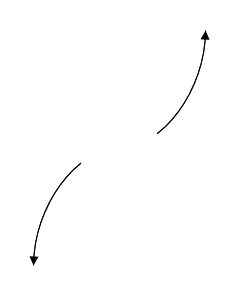
\includegraphics[width=0.3\textwidth]{../Figures/polyEndBehaviorCopyDA.png}
\end{center}\begin{enumerate}[label=\Alph*.]
\begin{multicols}{2}
\item 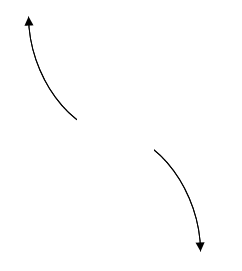
\includegraphics[width = 0.3\textwidth]{../Figures/polyEndBehaviorCopyAA.png}
\item 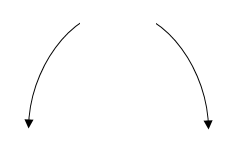
\includegraphics[width = 0.3\textwidth]{../Figures/polyEndBehaviorCopyBA.png}
\item 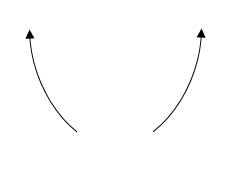
\includegraphics[width = 0.3\textwidth]{../Figures/polyEndBehaviorCopyCA.png}
\item 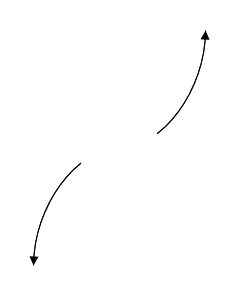
\includegraphics[width = 0.3\textwidth]{../Figures/polyEndBehaviorCopyDA.png}
\end{multicols}\item None of the above.\end{enumerate}
\textbf{General Comment:} Remember that end behavior is determined by the leading coefficient AND whether the \textbf{sum} of the multiplicities is positive or negative.
}
\litem{
Describe the zero behavior of the zero $x = 7$ of the polynomial below.
\[ f(x) = 2(x - 2)^{3}(x + 2)^{2}(x - 7)^{10}(x + 7)^{7} \]The solution is the graph below, which is option C.
\begin{center}
    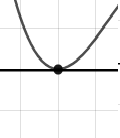
\includegraphics[width=0.3\textwidth]{../Figures/polyZeroBehaviorCA.png}
\end{center}\begin{enumerate}[label=\Alph*.]
\begin{multicols}{2}
\item 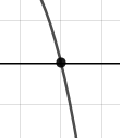
\includegraphics[width = 0.3\textwidth]{../Figures/polyZeroBehaviorAA.png}
\item 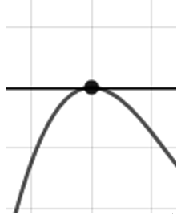
\includegraphics[width = 0.3\textwidth]{../Figures/polyZeroBehaviorBA.png}
\item 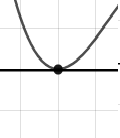
\includegraphics[width = 0.3\textwidth]{../Figures/polyZeroBehaviorCA.png}
\item 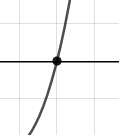
\includegraphics[width = 0.3\textwidth]{../Figures/polyZeroBehaviorDA.png}
\end{multicols}\item None of the above.\end{enumerate}
\textbf{General Comment:} You will need to sketch the entire graph, then zoom in on the zero the question asks about.
}
\litem{
Describe the zero behavior of the zero $x = 9$ of the polynomial below.
\[ f(x) = 2(x + 4)^{13}(x - 4)^{9}(x + 9)^{5}(x - 9)^{4} \]The solution is the graph below, which is option C.
\begin{center}
    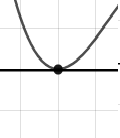
\includegraphics[width=0.3\textwidth]{../Figures/polyZeroBehaviorCopyCA.png}
\end{center}\begin{enumerate}[label=\Alph*.]
\begin{multicols}{2}
\item 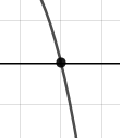
\includegraphics[width = 0.3\textwidth]{../Figures/polyZeroBehaviorCopyAA.png}
\item 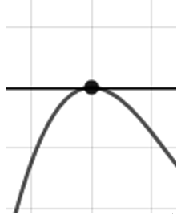
\includegraphics[width = 0.3\textwidth]{../Figures/polyZeroBehaviorCopyBA.png}
\item 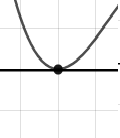
\includegraphics[width = 0.3\textwidth]{../Figures/polyZeroBehaviorCopyCA.png}
\item 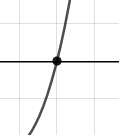
\includegraphics[width = 0.3\textwidth]{../Figures/polyZeroBehaviorCopyDA.png}
\end{multicols}\item None of the above.\end{enumerate}
\textbf{General Comment:} You will need to sketch the entire graph, then zoom in on the zero the question asks about.
}
\litem{
Which of the following equations \textit{could} be of the graph presented below?

\begin{center}
    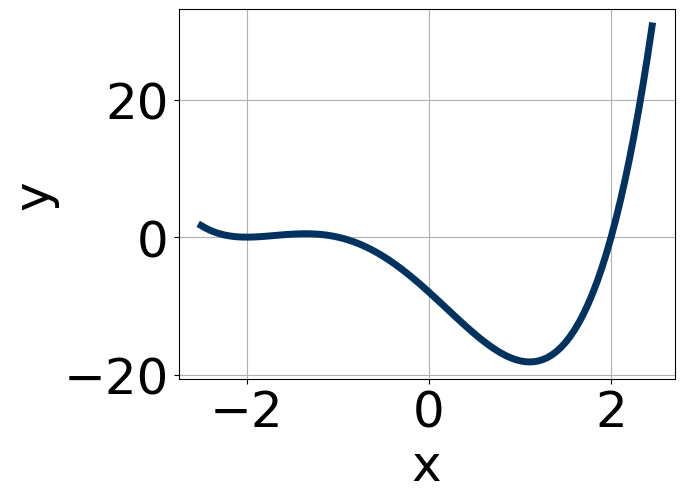
\includegraphics[width=0.5\textwidth]{../Figures/polyGraphToFunctionCopyA.png}
\end{center}


The solution is \( -15(x + 1)^{4} (x + 4)^{6} (x + 3)^{6} \), which is option C.\begin{enumerate}[label=\Alph*.]
\item \( -11(x + 1)^{6} (x + 4)^{11} (x + 3)^{7} \)

The factors $(x + 4)$ and $(x + 3)$ should both have even powers.
\item \( 18(x + 1)^{4} (x + 4)^{10} (x + 3)^{5} \)

The factor $(x + 3)$ should have an even power and the leading coefficient should be the opposite sign.
\item \( -15(x + 1)^{4} (x + 4)^{6} (x + 3)^{6} \)

* This is the correct option.
\item \( 19(x + 1)^{10} (x + 4)^{4} (x + 3)^{6} \)

This corresponds to the leading coefficient being the opposite value than it should be.
\item \( -15(x + 1)^{10} (x + 4)^{6} (x + 3)^{11} \)

The factor $(x + 3)$ should have an even power.
\end{enumerate}

\textbf{General Comment:} General Comments: Draw the x-axis to determine which zeros are touching (and so have even multiplicity) or cross (and have odd multiplicity).
}
\end{enumerate}

\end{document}